\chapter{Quantitative models: noise, RIN, and BER}
\label{ch:models}

The previous chapters argued mostly in architecture and measurement vocabulary.
This one puts numbers behind the two questions every link engineer eventually
asks: \emph{what bit-error ratio (BER) will this receiver deliver?} and
\emph{what is the minimum signal it needs?} The answers follow a short chain of
physics that has been stable for decades of IM/DD design: Gaussian statistics at
the decision circuit, a handful of noise sources, and the way relative intensity
noise (RIN) turns into an error floor. Understanding that chain is what lets you
read a sensitivity number or a RIN floor without treating the datasheet as magic.

Everything here is backed by short, reproducible Python (in \code{sims/}), so the
figures are computed curves rather than sketches. The models follow the treatment
in Säckinger's \emph{Analysis and Design of Transimpedance Amplifiers for Optical
Receivers},\sidenote{\citehref{sackinger2018}{E.~Säckinger, \emph{Analysis and Design of Transimpedance
Amplifiers for Optical Receivers}, Wiley, 2018, ch.~4}.} and the sanity checks in
the code reproduce that book's worked numbers.

\paragraph{Model-fidelity ladder.}
Use the simplest model that answers the decision. Do not force a simple model
to explain evidence outside its assumptions. This is a model-fidelity ladder,
not a product lifecycle.
\begin{description}
\item[Level 1. Scalar link budget] Tx OMA or power, path loss, receiver
      sensitivity, allocated penalties and margin. Answers: does the first-order
      budget close?
\item[Level 2. Equivalent-$Q$ noise model] Optical levels, responsivity,
      thermal/shot/RIN, effective noise bandwidth. Answers: does stochastic
      vertical noise explain the required BER?
\item[Level 3. Waveform and channel model] Finite bandwidth, dispersion,
      jitter, ISI, nonlinear levels, reflections, equalization, compression.
      Answers: how does the real waveform behave?
\item[Level 4. Measured statistical behavior] BER waterfalls, error
      histograms, time-correlated bursts, temperature and lane distributions.
      Answers: does the product population match the model?
\end{description}

\section{The decision: from \texorpdfstring{$Q$}{Q} to BER}
\label{sec:qber}

A binary receiver samples a noisy voltage and compares it to a threshold. If the
noise is Gaussian and the threshold is optimally placed, the BER depends on a
single quality factor $Q$, the separation between the one and zero levels
measured in units of their combined noise:
\[
  Q = \frac{I_1 - I_0}{\sigma_1 + \sigma_0},
  \qquad
  \mathrm{BER} = \tfrac{1}{2}\,\mathrm{erfc}\!\left(\frac{Q}{\sqrt{2}}\right).
\]
The mathematical $Q$-to-BER mapping depends on the sampled level distributions
rather than directly on the optical pulse shape. Pulse shape, bandwidth,
dispersion, jitter, and equalization still determine those distributions and
therefore cannot be ignored when predicting $Q$ from a physical link. This
binary $Q$-to-BER equation is an \emph{equivalent-quality} approximation used
throughout link budgeting. A full PAM4 treatment evaluates three decision
boundaries, unequal level noise, nonlinearity, equalization, and Gray mapping; do
not treat the binary formula as a complete PAM4 model. When applying the
approximation to a PAM4-class example, call it a \emph{binary-equivalent} $Q$.
\sidenote{$Q$ here is the electrical decision quality, not a laser-cavity or
resonator $Q$.} Two reference points anchor the binary curve: the classic uncoded
target $\mathrm{BER}=10^{-12}$ needs $Q=7.03$. For a named KP4-class optical PMD
under its random-error assumption, a pre-FEC objective near $2.4\times10^{-4}$
corresponds to $Q\approx3.5$ on this binary map (\Cref{ch:imdd}). That number is
not a universal Reed--Solomon threshold; state the FEC architecture, error model,
target PMD, and post-FEC metric.

\paragraph{BER and FEC terminology.}
Pre-FEC BER or symbol-error behavior describes the decoder input. Post-FEC
behavior describes residual errors after decoding. Corrected-codeword counts can
reveal declining margin before post-FEC failure. FEC thresholds depend on code,
interleaving, PMD, error distribution, and implementation. Burst errors can be
more harmful than an equal average random BER. A quoted FEC threshold is not a
universal analog receiver specification (\Cref{ch:networking,ch:imdd}).

\begin{lstlisting}
from scipy.special import erfc, erfcinv
import numpy as np

def q_to_ber(q):
    return 0.5 * erfc(q / np.sqrt(2))

def ber_to_q(ber):
    return np.sqrt(2) * erfcinv(2 * ber)
\end{lstlisting}

\begin{figure}[ht]
\centering
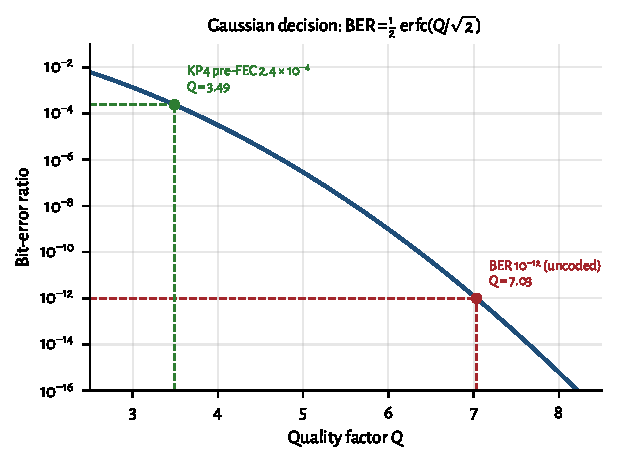
\includegraphics[width=\linewidth]{figures/fig_ber_vs_q.pdf}
\caption{The Gaussian decision curve. Every dB of $Q$ buys orders of magnitude of
BER near the knee, which is why FEC (trading a modest $Q$ for a huge BER
improvement) is decisive.\label{fig:berq}}
\end{figure}

\Cref{fig:berq} shows why the curve is so steep near the operating point: a small
change in $Q$ (equivalently, in received power) moves the BER by orders of
magnitude. This steepness is exactly what FEC exploits: nudging the required $Q$
from 7.03 down to 3.5 relaxes the optical power budget by several dB.

\section{The receiver noise budget}
\label{sec:noise}

$Q$ is only as good as our estimate of $\sigma$. Three noise sources dominate a
short-reach IM/DD receiver. Independent noise sources add in variance (equivalently,
rms amplitudes add in quadrature):

\begin{description}
\item[Thermal / circuit noise] the input-referred noise of the TIA and following
      stages, roughly white, so its variance scales with the noise bandwidth:
      $\sigma_{\text{th}}^2 = i_n'^2\,\mathrm{BW}$, where $i_n'$ is a noise-current
      density (A/$\sqrt{\text{Hz}}$). \emph{Signal-independent.}
\item[Shot noise] from the discreteness of photocurrent,
      $\sigma_{\text{shot}}^2 = 2q\,I\,\mathrm{BW}$. \emph{Grows with signal},
      so it is larger on the ones than the zeros.
\item[RIN (relative intensity noise)] the laser's own intensity fluctuations,
      $\sigma_{\text{RIN}}^2 = \mathrm{RIN}_{\text{lin}}\,I^2\,\mathrm{BW}$, with
      $\mathrm{RIN}_{\text{lin}} = 10^{\mathrm{RIN[dB/Hz]}/10}$.
      \emph{Grows with the square of signal}, the key fact of the next section.
\end{description}

\paragraph{Noise bandwidth.}
Noise bandwidth is the integral of the squared magnitude of the applicable noise
transfer function, expressed as an equivalent rectangular bandwidth. It is not
automatically equal to baud rate, bit rate, or the receiver's quoted $-3$~dB
bandwidth. A first-order estimate must name where the noise density is referred,
which filter response is assumed, and whether equalization changes the integrated
noise.

\paragraph{Limits of variance addition.}
Correlated sources need covariance terms. Discrete spurs should not be treated
automatically as white noise. Data-dependent jitter and ISI are not necessarily
stochastic noise. RIN altered by reflections may be frequency-dependent and
nonstationary. Receiver adaptation can change the effective noise transfer
function. Do not add thermal, shot, and RIN \emph{currents} as if they were
amplitudes on one line.

Because shot and RIN noise are signal dependent, we evaluate $\sigma_1$ and
$\sigma_0$ separately and form $Q$ with their sum. The core of the model is just
this:

\begin{lstlisting}
def nrz_q(p_avg_w, responsivity, i_thermal_rms, bw,
          er_db=np.inf, rin_db_hz=-np.inf):
    p1, p0 = er_levels(p_avg_w, er_db)      # one / zero optical powers
    i1, i0 = responsivity * p1, responsivity * p0
    var1 = i_thermal_rms**2 + 2*Q_E*i1*bw   # thermal + shot
    var0 = i_thermal_rms**2 + 2*Q_E*i0*bw
    if np.isfinite(rin_db_hz):
        rin = 10**(rin_db_hz / 10)
        var1 += rin * i1**2 * bw            # RIN grows as I^2
        var0 += rin * i0**2 * bw
    return (i1 - i0) / (np.sqrt(var1) + np.sqrt(var0))
\end{lstlisting}

\section{RIN and the BER floor}
\label{sec:rin}

Here is the consequence that makes RIN worth its own section. Thermal noise is
fixed, so pouring on more optical power raises $I_1-I_0$ while $\sigma_{\text{th}}$
stays put, so $Q$ improves without limit. But RIN noise scales \emph{with the signal
itself}: $\sigma_{\text{RIN}} \propto I$. Once RIN dominates, the signal and its
noise grow together and $Q$ stops improving. Taking the high-power, high-extinction
limit (thermal and shot negligible, $I_0\to0$):
\[
  Q_{\max} \;=\; \frac{I_1}{\sigma_{\text{RIN},1}}
           \;=\; \frac{1}{\sqrt{\mathrm{RIN}_{\text{lin}}\,\mathrm{BW}}}.
\]
This is a \emph{simplified dominant-RIN ceiling}, not a universal hard limit for
every PAM4 product. It assumes dominant RIN, a defined effective bandwidth,
approximately Gaussian stationary noise, adequate extinction, binary or idealized
level structure, no receiver overload, and no stronger jitter, ISI, reflection,
or nonlinear limitation. Under those assumptions, no amount of transmit power or
receiver sensitivity can push $Q$ past $Q_{\max}$, so a BER floor appears.
Equivalently, the power penalty to hold a target $Q$ is
\[
  \mathrm{PP} = \frac{1}{\sqrt{1 - Q^2\,\mathrm{RIN}_{\text{lin}}\,\mathrm{BW}}},
\]
which diverges as $Q\to Q_{\max}$.

\heuristic{If the waterfall floors, stop raising launch power as the primary
fix. You are buying photons against a non-power-limited impairment.}

\begin{figure}[ht]
\centering
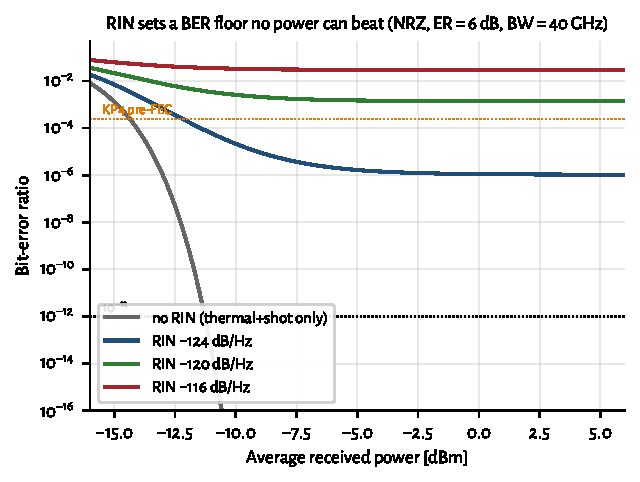
\includegraphics[width=\linewidth]{figures/fig_ber_vs_power_rin.pdf}
\caption{With RIN present, the BER stops falling no matter how much power is added.
The thermal/shot-only curve dives; each RIN level flattens into a floor. (RIN
values here are deliberately high to make the floor visible in-frame; good DFBs at
$<-150$~dB/Hz have no floor at these rates; see text.)\label{fig:berpower}}
\end{figure}

\begin{figure}[ht]
\centering
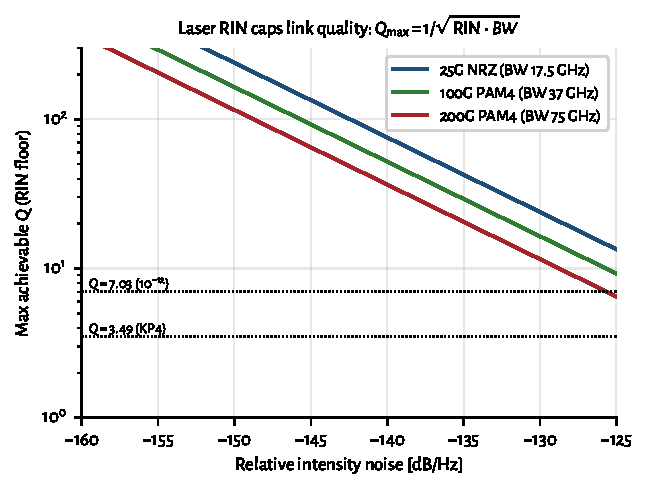
\includegraphics[width=\linewidth]{figures/fig_rin_floor.pdf}
\caption{The RIN ceiling $Q_{\max}=1/\sqrt{\mathrm{RIN}\cdot\mathrm{BW}}$. Wider
receiver bandwidth (higher lane rate) integrates more RIN, lowering the ceiling.
Where a curve dips below the dotted anchors, that link can no longer reach the
corresponding BER.\label{fig:rinfloor}}
\end{figure}

\Cref{fig:berpower} shows the floor directly; \Cref{fig:rinfloor} plots the ceiling
versus RIN for three lane rates. The bandwidth dependence matters: doubling the
lane rate doubles the noise bandwidth and drops $Q_{\max}$ by
$\sqrt{2}$ ($\approx1.5$~dB of margin), so RIN that is harmless at 25G can bite at
200G. This is the quantitative reason the laser chapter (\Cref{ch:lasers}) lists
RIN among the parameters that decide pass/fail.

\subsection{Typical RIN values (2026)}
\label{sec:rin-values}

How much RIN headroom do real sources have? \Cref{tab:rin-values} collects
representative figures. Two cautions on reading them. First, standards quote
\emph{$\mathrm{RIN}_x\mathrm{OMA}$}, RIN referenced to the OMA and measured under
a specified optical return loss (ORL) $x$, because back-reflections into the laser
raise its noise, so a spec limit is a stressed, worst-case number, not the
device's quiet intrinsic RIN.\sidenote{For example \citehref{rinspec}{IEEE~802.3 / 100G~Lambda~MSA
short-reach PAM4 links} cap $\mathrm{RIN}_{17.1}\mathrm{OMA}$ at $-136$~dB/Hz with
\SI{17.1}{dB} ORL~\cite{rinspec}.} Second, RIN degrades with optical feedback, so
isolator-free and co-packaged designs care as much about \emph{feedback tolerance}
as about the isolated number, one reason quantum-dot lasers (near-zero
linewidth-enhancement factor) are attractive for CPO~\cite{qdrin}.

A RIN number in dB/Hz is, by itself, incomplete: because RIN is \emph{relative},
it only becomes an absolute noise current once the photocurrent $I=\mathcal{R}P$
is fixed. The intensity-noise current density is
\[
  i_{\text{RIN}} = \sqrt{\mathrm{RIN}_{\text{lin}}}\;I \quad[\text{A}/\sqrt{\text{Hz}}],
  \qquad
  S_{\text{RIN}} = \mathrm{RIN}_{\text{lin}}\,I^2 \quad[\text{A}^2/\text{Hz}],
\]
so it scales linearly with received power. \Cref{tab:rin-values} therefore lists
both the RIN and the current density it produces at a common reference operating
point ($\mathcal{R}=0.8$~A/W, $P_{\text{rx}}=0$~dBm, i.e.\ $I=0.8$~mA), the units a
receiver designer actually compares against.

\begin{table*}[ht]
\refstepcounter{table}\label{tab:rin-values}%
\centering
\setlength{\tabcolsep}{4pt}%
\renewcommand{\arraystretch}{1.25}%
\begin{tabular}{@{}p{0.26\linewidth}p{0.12\linewidth}p{0.18\linewidth}p{0.12\linewidth}p{0.18\linewidth}@{}}
\toprule
Source & RIN (dB/Hz) & $i_{\text{RIN}}$ @ 0 dBm & Metric & Note \\
\midrule
400G-FR4 / 100G Lambda class limit & $\le -136$ & $\ge 127$ & stressed $\mathrm{RIN}_x\mathrm{OMA}$ & named ORL (e.g.\ 17.1~dB) \\
\addlinespace[1.5em]
Datacom VCSEL, 850~nm (MMF) & $-135$ to $-145$ & $45$ to $142$ & intrinsic & quiet parts $\le\!-145$ \\
\addlinespace[1.5em]
Good datacom DFB / EML & $-145$ to $-155$ & $14$ to $45$ & intrinsic & CPO ELS often target $\le\!-145$ \\
\addlinespace[1.5em]
Quantum-dot laser on Si & $-140$ to $-150$ & $25$ to $80$ & intrinsic & feedback-tolerant class \\
\addlinespace[1.5em]
Heterogeneous / injection-locked Si & $-155$ to $-165$ & $4.5$ to $14$ & intrinsic & high-$Q$ feedback \\
\addlinespace[1.5em]
Lab record (QD + injection lock) & $\sim\!-168$ & $\sim 3.2$ & intrinsic & research \\
\bottomrule
\end{tabular}
\par\medskip
{\raggedright\footnotesize\textbf{Table~\thetable.} Representative RIN by source
(c.~2026) at $\mathcal{R}=0.8$~A/W, $P_{\text{rx}}=0$~dBm ($I=0.8$~mA). Intrinsic
RIN and stressed $\mathrm{RIN}_x\mathrm{OMA}$ are different metrics; do not convert
them through one equation unless the definitions align. Density
$i_{\text{RIN}}=\sqrt{\mathrm{RIN}_{\text{lin}}}\,I$.\par}
\end{table*}

For scale, at that same $0.8$~mA the \emph{shot}-noise density is
$\sqrt{2qI}=16$~pA/$\sqrt{\text{Hz}}$ ($S=2.6\times10^{-22}$~A$^2$/Hz) and a good
high-speed TIA adds roughly $25$~pA/$\sqrt{\text{Hz}}$ of thermal noise. So a VCSEL
at $-140$~dB/Hz ($80$~pA/$\sqrt{\text{Hz}}$) already dominates both, while a
heterogeneous source at $-160$~dB/Hz ($8$~pA/$\sqrt{\text{Hz}}$) is a minor term.
The key asymmetry: thermal noise is fixed and shot grows only as $\sqrt{I}$, but
RIN grows as $I$, so at low received power thermal wins and RIN is irrelevant, and
only above a break-in power (\Cref{fig:noisedensity}) does RIN take over. That is
why quoting a RIN figure without an operating power says little.

\begin{figure}[ht]
\centering
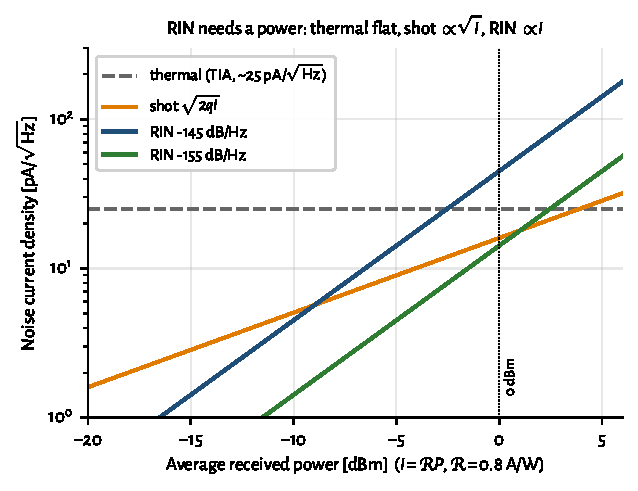
\includegraphics[width=\linewidth]{figures/fig_noise_density_vs_power.pdf}
\caption{Noise current densities versus received power. Thermal is flat, shot
$\propto\!\sqrt{I}$, RIN $\propto\!I$; the RIN curves cross the fixed thermal floor
only above a break-in power, which is why RIN only ``makes sense'' once the optical
power (hence $I=\mathcal{R}P$) is stated.\label{fig:noisedensity}}
\end{figure}

Put these against the simplified dominant-RIN ceiling
$Q_{\max}=1/\sqrt{\mathrm{RIN}\cdot\mathrm{BW}}$. Assumptions: RIN dominates,
noise bandwidth is defined, level structure is idealized, no stronger
deterministic impairment is present, and the receiver is not compressed. At
200G-PAM4 bandwidths ($\mathrm{BW}\approx75$~GHz), plugging the stressed
$-136$~dB/Hz $\mathrm{RIN}_x\mathrm{OMA}$ number into that intrinsic-style formula
is illustrative only; the definitions do not automatically align. Even under that
optimistic plug-in, $Q_{\max}\approx23$ is far above $Q=7$ for $10^{-12}$, so for
well-behaved sources RIN is often not the limiter; thermal noise is. RIN becomes
the story when feedback, aging, or a marginal source pushes the \emph{effective}
intensity noise toward $-125$~dB/Hz class. A third path is electrical: laser
bias-driver current noise converts to equivalent RIN
(\Cref{sec:laser-drivers}) and must be budgeted separately from intrinsic laser
RIN.

\begin{table*}[ht]
\refstepcounter{table}\label{tab:rin-metric-defs}%
\centering
\setlength{\tabcolsep}{3pt}%
\footnotesize
\renewcommand{\arraystretch}{1.2}%
\begin{tabular}{@{}p{0.28\linewidth}p{0.68\linewidth}@{}}
\toprule
Quantity & Meaning \\
\midrule
Intrinsic RIN & Relative intensity-noise spectrum under stated source conditions \\
\addlinespace[0.8em]
Stressed $\mathrm{RIN}_x\mathrm{OMA}$ & Standard-defined Tx metric under a named ORL and normalization \\
\addlinespace[0.8em]
Equivalent bias-board RIN & Optical intensity noise from electrical current-noise coupling \\
\addlinespace[0.8em]
Absolute RIN current density & Current-noise density at a stated photocurrent \\
\bottomrule
\end{tabular}
\par\medskip
{\raggedright\footnotesize\textbf{Table~\thetable.} RIN-related quantities. Similar
units do not guarantee identical definitions
(\Cref{sec:laser-drivers,ch:lasers}).\par}
\end{table*}

\keyidea{Thermal noise is beaten by power; dominant RIN is not. Under a
simplified model, $\sigma_{\text{RIN}}\propto I$ imposes
$Q_{\max}=1/\sqrt{\mathrm{RIN}\cdot\mathrm{BW}}$. Keep intrinsic RIN and stressed
$\mathrm{RIN}_x\mathrm{OMA}$ separate. Feedback, aging, and bias-board noise erode
the margin that quiet intrinsic sources appear to have.}

\section{Sensitivity and OMA}
\label{sec:sensitivity}

\subsection{Common misconception: sensitivity does not guarantee a working link}

Received power exceeding the datasheet sensitivity number does not guarantee low
BER. Sensitivity is measured under specific, controlled assumptions: a clean
transmitter, known extinction ratio, specified ORL, and a particular equalization
state. In the field, BER depends on all of these simultaneously:

\begin{itemize}
\item received optical power;
\item extinction ratio and OMA (not just average power);
\item RIN under the actual ORL;
\item jitter (random and deterministic);
\item ISI from bandwidth limits and dispersion;
\item receiver thermal noise and any TIA compression;
\item equalization state and FEC margin.
\end{itemize}

Sensitivity is therefore a shorthand for receiver noise performance under reference
conditions, not a complete description of whether the link closes. A link that
``has enough power'' can still fail if ER is poor, RIN is elevated, or the
equalizer is saturated. Always close the full link budget
(\Cref{sec:link-budget}), not just the power line.

\begin{table*}[ht]
\refstepcounter{table}\label{tab:metric-planes}%
\centering
\setlength{\tabcolsep}{3pt}%
\footnotesize
\renewcommand{\arraystretch}{1.2}%
\begin{tabular}{@{}p{0.22\linewidth}p{0.74\linewidth}@{}}
\toprule
Quantity & Required condition \\
\midrule
Transmit average power & Named output plane and operating state \\
\addlinespace[0.7em]
Transmit OMA & Named output plane, modulation definition, calibration method \\
\addlinespace[0.7em]
Received power & Receiver optical-input plane \\
\addlinespace[0.7em]
Receiver sensitivity & Average power or OMA; BER/FEC target; Tx condition; wavelength; temperature \\
\addlinespace[0.7em]
RIN & Intrinsic or stressed definition; optical power or OMA; ORL; frequency range \\
\addlinespace[0.7em]
TIA noise & Density or integrated rms; input reference; bandwidth and loading \\
\addlinespace[0.7em]
BER & Pre- or post-FEC; interval; pattern or traffic; lane and direction \\
\bottomrule
\end{tabular}
\par\medskip
{\raggedright\footnotesize\textbf{Table~\thetable.} Metric and reference-plane
checklist. A number without its metric definition and reference plane cannot be
entered safely into the model.\par}
\end{table*}

\tradeoff{Better receiver sensitivity vs receiver complexity}{APD gain, stronger
DSP, deeper equalization, or quieter optics can close a tight budget}{Power,
latency, calibration burden, and reliability of the more complex path}{When the
sensitivity line is the true limiting ledger after Tx and plant are sound}{Improve
the weakest link, not the most visible datasheet metric.}

\subsection{OMA versus average power}

Two links may have identical average optical power but different BER. The reason
is OMA and extinction ratio. At fixed average power $P_\mathrm{avg}$, the OMA
depends on ER through
\[
  \frac{\mathrm{OMA}}{P_\mathrm{avg}}
  = \frac{2(\mathrm{ER}-1)}{\mathrm{ER}+1},
\]
where ER is the linear extinction ratio $P_1/P_0$. A link with 10~dB ER
($\mathrm{ER}_\mathrm{lin}=10$) delivers
$\mathrm{OMA}/P_\mathrm{avg} = 18/11 \approx 1.636$, while 6~dB ER
($\mathrm{ER}_\mathrm{lin}\approx 4$) delivers $6/5 = 1.200$. The difference is
about 1.36~dB of OMA at the same average power. Whether that 1.36~dB matters
depends on where the receiver sits on its BER waterfall: near the sensitivity
cliff a 1~dB OMA change moves BER by orders of magnitude
(\Cref{sec:qber,fig:berpower}), while well above sensitivity the same change is
invisible. The impact also depends on RIN, bandwidth, equalization state, and
TDECQ; ER alone does not set BER.

For PAM4, the relevant quantity is the outer OMA ($P_3 - P_0$), and level spacing
(RLM) matters independently. A transmitter that launches adequate average power but
has compressed inner eyes (poor RLM) will fail TDECQ even though a power meter
reads in-spec. This is why TDECQ, OMA, and RLM are specified together, not average
power alone (\Cref{sec:tdecq}).

\subsection{The sensitivity formula}

Turning the question around (\emph{what is the least power that meets a target
BER?}) gives the sensitivity. Referring the receiver's input noise current
$i_n$ (already integrated rms, not a density) back to the optical input through
the responsivity $\mathcal{R}$:
\[
  P_{\text{sens}} = \frac{Q\,i_n}{\mathcal{R}}
  \qquad\text{(average power)},\qquad
  P_{\text{sens}}^{\text{OMA}} = \frac{2\,Q\,i_n}{\mathcal{R}}.
\]
These simple expressions assume binary signaling, a stated relation between
average power and OMA, high or explicitly handled extinction ratio,
signal-independent effective rms noise for the simplified form, a linear
detector and TIA, no substantial ISI, jitter, compression, or RIN floor, and an
optimal or defined decision threshold. For PAM4, treat the calculation as a
\emph{first-order binary-equivalent estimate}, not a standards-compliance
receiver calculation. A noise density in A/$\sqrt{\mathrm{Hz}}$ must be
integrated through the effective noise bandwidth before it enters these
equations.

Modern short-reach standards specify \term{OMA} rather than average power. For
binary NRZ, $\mathrm{OMA}=P_1-P_0$; for PAM4, outer OMA is $P_3-P_0$. OMA
decouples the sensitivity spec from extinction ratio. As a check, the textbook
example ($i_n = 1~\mu$A, $\mathcal{R}=0.8$~A/W, $\mathrm{BER}=10^{-12}$) gives
$P_{\text{sens}}=7.03\times1~\mu\text{A}/0.8 = 8.8~\mu$W, or $-20.6$~dBm, which
the code reproduces. A finite extinction ratio costs an idealized further
$\mathrm{PP}_\mathrm{dB}=10\log_{10}[(\mathrm{ER}_\mathrm{lin}+1)/(\mathrm{ER}_\mathrm{lin}-1)]$:
$0.87$~dB at 10~dB ER, $2.2$~dB at 6~dB ER. These penalties feed link budgets
(\Cref{ch:imdd}) and TDECQ discussion (\Cref{ch:validation}); do not double-count
TDECQ as an independent penalty if the compliance method already includes it. Do
not convert every impairment into arbitrary dB, mix average-power sensitivity
with OMA penalties, or combine nominal values from one plane with worst-case
values from another as if they were independent.

\paragraph{Worked example: DR4-class budget check.}
\label{sec:worked-budget}

Take a 200G/lane DR-class estimate with Ge-on-Si PIN ($\mathcal{R}=0.9$~A/W), TIA
$i_n=13$~pA/$\sqrt{\text{Hz}}$, noise bandwidth $\approx60$~GHz, and a KP4-class
pre-FEC objective $2.4\times10^{-4}$ mapped to binary $Q\approx3.5$
(\Cref{sec:qber,sec:kp4}). Reference plane: receiver optical input. Assume
Gaussian noise, equalized eye, no compression, and RIN not yet dominant.

Integrated thermal-class noise: $i_n \sqrt{\mathrm{BW}} \approx
13\times10^{-12}\times\sqrt{60\times10^9} \approx 3.2~\mu$A rms. Required OMA
under the binary sensitivity formula:
\[
P_{\text{OMA,sens}} = \frac{2 Q i_n \sqrt{\mathrm{BW}}}{\mathcal{R}}
\approx \frac{2\times3.5\times3.2~\mu\text{A}}{0.9} \approx 25~\mu\text{W}
\approx -16~\text{dBm}.
\]
Illustrative allocations (not a normative budget): $\sim$3~dB TDECQ-class Tx
impairment \emph{or} remaining margin after a TDECQ-based OMA method (not both),
$\sim$2~dB connector/fiber at stated planes, $\sim$2~dB system margin. That lands
near $-9$~dBm class OMA at the receiver input, or roughly $-6$ to $-4$~dBm
launched depending on reach. Parameter sensitivity: $\pm$1~dB in $i_n$ or
$\mathcal{R}$ moves the estimate about 1~dB; a RIN floor or MPI can invalidate
the waterfall entirely.

Where the model stops: unequal PAM4 levels, level-dependent noise, strong ISI,
compressed TIA, correlated RIN, or a different FEC/error model. If measured
sensitivity is worse, bisect RIN, reflections, and ER
(\Cref{sec:link-budget,sec:optical-channel}).

\paragraph{Model-validity checklist.}
Before applying $Q$, $Q_{\max}$, or $P_{\mathrm{sens}}$, ask:
\begin{itemize}
\item Is the noise approximately Gaussian at the decision point?
\item Is the noise bandwidth defined for this measurement?
\item Are PAM4 levels equally spaced (or is RLM budgeted)?
\item Is noise level-dependent (shot/RIN) accounted for?
\item Is the receiver compressed or overloaded?
\item Is residual ISI deterministic rather than noise-like?
\item Is RIN intrinsic, stressed $\mathrm{RIN}_x\mathrm{OMA}$, or bias-board noise?
\item Is the FEC threshold appropriate for this PMD and error model?
\item Is the input metric average power or OMA, and at which reference plane?
\end{itemize}

\begin{dectree}
Measured BER behavior
  |
Gaussian stationary waterfall?
  |-- YES --> equivalent-Q model may be adequate
  |-- NO  --> inspect PAM4 levels, ISI, jitter,
              bursts, reflections, compression,
              adaptation, and non-Gaussian tails
\end{dectree}

\paragraph{Correlating the model with the bench.}
\label{sec:model-to-bench}
A model is validated by prediction across changed conditions, not by fitting one
curve after the fact. Recommended order:
\begin{enumerate}
\item Verify attenuator and power-meter calibration.
\item Establish the optical reference plane.
\item Measure transmitter average power, OMA, ER or RLM, and quality metric.
\item Measure receiver noise or infer an effective value from trusted
      characterization.
\item Sweep received OMA and record BER with sufficient error count or dwell.
\item Fit only physically meaningful parameters.
\item Compare curve crossing, slope, floor, and overload behavior.
\item Repeat across lanes and temperature.
\item Record model uncertainty and measurement uncertainty separately.
\end{enumerate}

\section{Receiver technologies and their noise (2026)}
\label{sec:rxtech}

The sensitivity formula $P_{\text{sens}}=Q\,i_n/\mathcal{R}$ has exactly two
device inputs: the photodiode responsivity $\mathcal{R}$ and the amplifier's
input-referred noise current $i_n$. So ``receiver noise performance'' is really a
statement about the detector--TIA pair. Ge-on-silicon PIN plus a closely
integrated CMOS or SiGe TIA is a common short-reach path because it offers useful
responsivity, bandwidth, and integration. Alternative detectors become attractive
when gain, saturation, wavelength, linearity, or packaging requirements change
(\Cref{sec:pd-tia}).

\paragraph{Photodiodes and transimpedance amplifiers.}
\label{sec:pd-tia}

The photodiode converts photons to photocurrent; the \term{TIA}\firstterm{TIA}
(transimpedance amplifier) converts current to voltage with low input-referred noise.
For PAM4 at 100--224G/lane:

\begin{itemize}
\item \textbf{PIN (Ge-on-Si):}\firstterm{PIN} no internal gain; lowest excess noise; common
      short-reach choice (\Cref{tab:rxtech}). Capacitance at the TIA input dominates
      $i_n$.
\item \textbf{APD}\firstterm{APD}: internal multiplication. Any sensitivity benefit versus
      PIN depends on gain, excess-noise factor, bandwidth, receiver design, and BER
      target; published Ge/Si APD results often cite roughly 5--9~dB under specific
      conditions, not as a universal gain~\cite{apd}.
\item \textbf{UTC/MUTC:}\firstterm{UTC} electron-only transport for $>\!200$~GHz BW and high
      saturation; used when linearity and speed beat raw sensitivity~\cite{utc}.
\end{itemize}

The TIA often embeds \term{CTLE} for LPO (\Cref{sec:equalization,sec:conditioning}):
a fixed high-frequency boost before the host SerDes ADC. Co-packaging PD and TIA
(sub-mm interconnect) is the noise win repeated throughout this book
(\Cref{ch:firstprinciples}).

\paragraph{Why Ge-on-Si is a common mainstream path.} Germanium grown on silicon
absorbs the O- and C-bands, is CMOS-process-compatible, and can be built on the
same PIC as the modulators and couplers. Modern devices reach
$\mathcal{R}\approx0.8$--$1.0$~A/W with dark currents of single-digit to tens of
nA and, in mid-2020s research, $-3$~dB bandwidths beyond 100~GHz (e.g.\ a recessed
Ge/Si PIN at 106~GHz, $0.93$~A/W, $<10$~nA; SiN-coupled lateral Ge $>110$~GHz at
1~mA)~\cite{gesipd}. Monolithic or 3D/flip-chip co-integration keeps the
PD-to-TIA interconnect short, so the input node capacitance stays low. In common
front-end-limited approximations, input-referred noise rises strongly with input
capacitance and required bandwidth; some simplified architectures produce an
approximate $i_n \!\propto\! C\,f^{3/2}$ scaling. Actual scaling depends on TIA
topology, transistor technology, feedback network, detector impedance,
equalization, power, and stability. Short interconnects remain quiet when those
terms cooperate (\Cref{ch:firstprinciples}).

\paragraph{What the TIA must deliver.}
\label{sec:tia-specs}

The TIA is the receive twin of the modulator driver (\Cref{sec:drivers}). At
224~GBd PAM4 you need bandwidth $\gtrsim$50--70~GHz for a 112~GBd Nyquist-class
front-end (often less than the Tx driver BW because the optical channel and
reference receiver already band-limit; LPO pushes for flatter, more linear TIAs),
input-referred noise in the low teens of pA$/\sqrt{\mathrm{Hz}}$ once co-packaged
with a low-$C$ PD, linearity / overload so large OMA and reflections do not crush
PAM4 levels (RLM) or trip AGC into a bad corner, and optional CTLE for LPO/LRO so
the host SerDes sees a usable eye without module DSP
(\Cref{sec:equalization,sec:conditioning}).
In common front-end-limited approximations, noise rises strongly with input
capacitance and bandwidth (sometimes near $i_n \propto C\,f^{3/2}$). That is why
close detector--TIA integration is valuable at 200G+: every millimetre of
bondwire spends noise and bandwidth that FEC cannot recover. Integration is an
engineering trade against repairability and yield, not a universal mandate.

\paragraph{Noise levels you actually budget.}
\Cref{tab:tia-noise} puts the model numbers next to published front-ends. Shot noise
at 0~dBm into $\mathcal{R}=0.8$~A/W is $\sqrt{2qI}\approx16$~pA$/\sqrt{\mathrm{Hz}}$;
a good TIA sits near that floor. Worse $i_n$ or higher $C$ burns sensitivity
linearly via $P_{\mathrm{sens}}=Q\,i_n/\mathcal{R}$ (\Cref{sec:sensitivity}).

\begin{table*}[ht]
\refstepcounter{table}\label{tab:tia-noise}%
\centering
\setlength{\tabcolsep}{3.5pt}%
\footnotesize
\renewcommand{\arraystretch}{1.25}%
\begin{tabular}{@{}p{0.28\linewidth}p{0.18\linewidth}p{0.22\linewidth}p{0.24\linewidth}@{}}
\toprule
Front-end & $i_n$ (pA$/\sqrt{\mathrm{Hz}}$) & BW / rate & Sensitivity note \\
\midrule
Typical ``good'' short-reach TIA (book model) & $\sim$25 & --- & older rule-of-thumb floor \\
\addlinespace[1.5em]
16-nm CMOS + co-pkg PD & 16.9 & 32~GHz / 112G PAM4 & $-8.2$~dBm class \\
\addlinespace[1.5em]
55-nm SiGe $4\times$112~GBd linear TIA & 13.2 & 65~GHz / 224G & $\sim$1.2~pJ/bit \\
\addlinespace[1.5em]
Shot noise @ 0~dBm, $\mathcal{R}=0.8$~A/W & $\approx$16 & --- & physics floor at that power \\
\bottomrule
\end{tabular}
\par\medskip
{\raggedright\footnotesize\textbf{Table~\thetable.} Input-referred TIA noise densities
used in link budgets (c.~2023--26 published front-ends). Integrate $i_n\sqrt{\mathrm{BW}}$
for rms noise before applying $Q$ (\Cref{sec:sensitivity}). Sources in text.\par}
\end{table*}

2026 linear PAM4 front-ends land around $10$--$17$~pA$/\sqrt{\text{Hz}}$: e.g.\
$16.9$~pA$/\sqrt{\text{Hz}}$ at 112G in 16-nm CMOS ($-8.2$~dBm
sensitivity)~\firstcite{tia112} and $13.2$~pA$/\sqrt{\text{Hz}}$ at 224G in
55-nm SiGe BiCMOS (65~GHz BW, 1.2~pJ/bit)~\firstcite{tia224}. Put these in the
model: $i_n\approx13$~pA$/\sqrt{\text{Hz}}$ integrated over $\sim\!60$~GHz is
$\approx3.2~\mu$A rms, giving an NRZ average sensitivity near $-15$~dBm; the PAM4
level penalty lands OMA sensitivities in the $-8$ to $-10$~dBm range these
front-ends report.

\paragraph{Industry snapshot --- mid-2026 (receivers).}
\Cref{tab:rx-records} pairs detectors and TIAs with maturity labels. Commercial
linear-optics TIAs (Semtech GN1834L/DL, GN1838DL) target LPO/LRO/CPO at 224G/lane
with on-chip EQ (production / sampling class). Semtech has also shown 448G-class
PMD ICs (TN14740 TIA) at OFC~2026 demos (vendor demonstration; not a volume
datasheet claim)~\firstcite{semtech224,semtech448demo}. On the detector side,
recessed Ge/Si PINs at 106~GHz / 0.93~A/W~\cite{gesipd}, Ge/Si UMC-APDs at
105~GHz with a published $\sim$9~dB sensitivity gain over PIN at 224/260G PAM4
under that paper's conditions~\firstcite{apd}, waveguide Ge/Si APDs toward
100~GHz at 2~A/W~\firstcite{gesiapd100}, and OFC~2026 Ge-on-Si APDs at 180~GBd
PAM4~\firstcite{ofc360apd} mark the research edge. UTC/MUTC PDs remain the
high-saturation / $>\!200$~GHz niche~\cite{utc}.

\begin{table*}[ht]
\refstepcounter{table}\label{tab:rx-records}%
\centering
\setlength{\tabcolsep}{3pt}%
\footnotesize
\renewcommand{\arraystretch}{1.25}%
\begin{tabular}{@{}p{0.26\linewidth}p{0.14\linewidth}p{0.16\linewidth}p{0.18\linewidth}p{0.18\linewidth}@{}}
\toprule
Part / paper & Type & BW / $i_n$ or $\mathcal{R}$ & Rate / sens. & Note \\
\midrule
Semtech GN1834L/DL / GN1838DL & TIA & 224G-class; linear+EQ & 224~Gb/s/lane & Commercial LPO/CPO family \\
\addlinespace[1.5em]
Semtech TN14740 (demo) & TIA & 448G-class & 448G/lane demo & OFC 2026 booth; provisional \\
\addlinespace[1.5em]
SiGe $4\times$112~GBd TIA & TIA & 65~GHz; 13.2~pA$/\sqrt{\mathrm{Hz}}$ & 224G PAM4 & Research / product-class paper \\
\addlinespace[1.5em]
16-nm CMOS + co-pkg PD & TIA+PD & 16.9~pA$/\sqrt{\mathrm{Hz}}$ & 112G; $-8.2$~dBm & Co-packaged win \\
\addlinespace[1.5em]
Recessed Ge/Si PIN & PD & 106~GHz; 0.93~A/W & 200~GBd-class & $<$10~nA dark \\
\addlinespace[1.5em]
Ge/Si UMC-APD & APD & 105~GHz @ $M\!\approx\!7$ & 224/260G; $-10.9$/$-10.1$~dBm & $\sim$9~dB over PIN (paper conditions) \\
\addlinespace[1.5em]
Ge/Si WG APD (300~mm) & APD & $>$100~GHz; 2~A/W @ 70~GHz & 400G/lane target & 7~V bias class \\
\addlinespace[1.5em]
OFC 2026 Ge-on-Si APD & APD & 70--100~GHz; 1.5--2~A/W & 180~GBd PAM4 & O- and C-band \\
\addlinespace[1.5em]
UTC / MUTC-PD & PD & $>\!110$--200~GHz & high $I_{\mathrm{sat}}$ & Linear / LPO niche \\
\bottomrule
\end{tabular}
\par\medskip
{\raggedright\footnotesize\textbf{Table~\thetable.} Receiver snapshot (c.~2025--26).
Commercial TIA rows are vendor announcements; APD/PIN rows mix production-intent
SiPh with research demos. Sensitivities are as published (FEC threshold varies).\par}
\end{table*}

\paragraph{Reasonable alternatives to Ge PIN + quiet TIA.}
\Cref{tab:rxtech} lays the detector menu out. III-V InGaAs PINs (flip-chipped)
trade monolithic integration for higher power handling and remain common in
discrete modules. Avalanche photodiodes add internal gain that can improve sensitivity when gain,
excess noise, bandwidth, and BER target cooperate (published short-reach results
often land near 5--9~dB under specific conditions) at the cost of bias complexity
and excess noise; device bandwidth above 100~GHz is no longer rare in
research~\cite{apd,gesiapd100,ofc360apd}.
Uni-traveling-carrier (UTC/MUTC) PDs use electron-only transport for very high
saturation current, linearity, and bandwidth ($>\!200$~GHz) but modest
responsivity, a fit for linear/LPO and $>\!200$~GBd analog optics more than for
raw sensitivity~\cite{utc}. SOA\firstterm{SOA}-preamplified receivers bolt optical gain ahead of
the PD for large effective responsivity and reach, but pay in ASE noise figure,
power, and complexity.

\begin{table*}[ht]
\refstepcounter{table}\label{tab:rxtech}%
\centering
\setlength{\tabcolsep}{5pt}%
\footnotesize
\renewcommand{\arraystretch}{1.25}%
\begin{tabular}{@{}p{0.22\linewidth}p{0.13\linewidth}p{0.15\linewidth}p{0.16\linewidth}p{0.21\linewidth}@{}}
\toprule
Detector & $\mathcal{R}$ (A/W) & $-3$~dB BW & Integration & Where it fits \\
\midrule
Ge-on-Si waveguide PIN & $0.8$--$1.0$ & $60$--$>\!100$~GHz & monolithic on SiPh & mainstream short-reach / CPO \\
\addlinespace[1.5em]
III-V InGaAs PIN (flip-chip) & $0.6$--$0.9$ & $60$--$>\!100$~GHz & hybrid / flip-chip & discrete modules, high power \\
\addlinespace[1.5em]
APD (Ge/Si, InP, UMC) & effective $\uparrow$ (gain) & up to $\sim\!100$~GHz+ & hybrid / emerging & power-starved links; gain benefit condition-dependent \\
\addlinespace[1.5em]
UTC / MUTC-PD & $0.1$--$0.8$ & $>\!110$--$200$~GHz & III-V & linear/LPO, $>\!200$~GBd, high saturation \\
\addlinespace[1.5em]
SOA-preamplified PD & effective $\gg\!1$ & $\sim\!50$~GHz & III-V PIC & tight power budgets; adds ASE noise \\
\bottomrule
\end{tabular}
\par\medskip
{\raggedright\footnotesize\textbf{Table~\thetable.} Short-reach receiver detector
options, c.~2026. Ranges span production to recent research; APD/UTC/SOA figures
are effective (with gain) or device-record.\par}
\end{table*}

\paragraph{Outlook.}
Volume short-reach receive commonly stays on PIN + SiGe/CMOS TIA: noise in the
low teens of pA$/\sqrt{\mathrm{Hz}}$ with $>\!100$~GHz Ge PINs is often enough
for DR/FR PAM4 when closely integrated, so the fight is capacitance and yield as
much as detector physics.
Linear optics raises the bar: LPO/LRO need high linearity, on-chip EQ, and
multi-lane density (Semtech's 224G family is the public commercial marker; 448G
TIA demos are still provisional, \Cref{sec:drivers}). APDs are back in the 200G
conversation when several dB of sensitivity gain changes a power-limited plant;
UTC/MUTC matter when the impairment is saturation or $>\!200$~GBd analog fidelity
rather than photons per bit. Bondwire and FAU still set $C$ and BW, which is why
CPO/NPO win on noise for the same reason they win on energy
(\Cref{ch:firstprinciples}).

\keyidea{Receiver performance is $\mathcal{R}$ and $i_n$, with $i_n$ set by PD+TIA
capacitance. Budget $10$--$17$~pA$/\sqrt{\mathrm{Hz}}$ co-packaged TIAs and
$>\!100$~GHz Ge PIN/APD detectors; use APD gain or UTC saturation when the link
demands it. LPO makes TIA linearity as important as raw noise.}

\section{NRZ versus PAM4, at equal bit rate}
\label{sec:nrzpam4}

The 224G-per-lane roadmap (\Cref{ch:imdd}) rides on PAM4, so it is worth seeing
the trade quantitatively. PAM8 and the full multilevel design argument live in
\Cref{ch:multilevel}. At equal bit rate, PAM4 halves the ideal symbol rate
relative to NRZ but divides the available outer modulation span among three eyes.
The resulting link penalty depends on bandwidth, transmitter linearity, level
spacing, level-dependent noise, equalization, coding, and FEC. The figure
$20\log_{10}3 \approx 9.5$~dB is an \emph{ideal vertical level-separation
comparison} before bandwidth and implementation effects. \Cref{fig:pam4} pits the
two at a common 100~Gb/s: PAM4's narrower bandwidth partly offsets its level
penalty, but it still often needs several dB more received power for the same
BER, repaid by relaxing the electrical bandwidth the SerDes and optics must
support. That balance is why many 100G/lane products used NRZ and 200G/lane
products used PAM4.

\begin{figure}[ht]
\centering
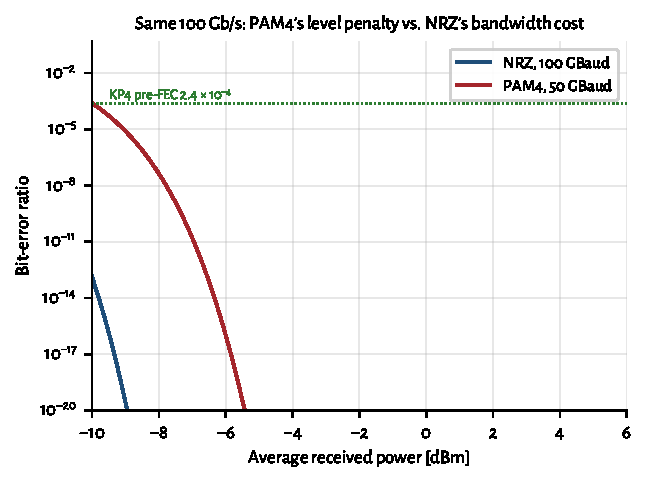
\includegraphics[width=\linewidth]{figures/fig_nrz_vs_pam4.pdf}
\caption{NRZ (100~GBaud) versus PAM4 (50~GBaud) at the same 100~Gb/s. PAM4 pays a
level penalty but relaxes bandwidth; the crossover with the KP4 pre-FEC threshold
sets the required operating power.\label{fig:pam4}}
\end{figure}

\section{Engineering lens}
\label{sec:models-engineering-lens}

\subsection{How it works}

Binary link models often collapse receiver performance to a quality factor $Q$:
signal separation divided by combined noise. That is a useful equivalent-quality
map, not a complete PAM4 theory. Thermal noise yields to more power; dominant RIN
does not, which is why a BER floor can exist. The rest of this chapter computes,
measures, and defends $Q$ under stated assumptions.

\subsection{How it is measured}
\label{sec:models-how-measured}

A BER model earns trust only when every term has a bench measurement. Use a BERT
and calibrated optical attenuator for BER versus received OMA. Measure receiver
input-referred noise with the photodiode dark and illuminated. Use a DCA for OMA,
ER, and eye quality, and a photodiode plus electrical spectrum analyzer for
relative intensity noise (RIN). Repeat power sweeps at temperature and per lane.
Acceptance is a curve, not one point: the required waterfall must cross the
program's pre-FEC threshold with margin and without a floor
(\Cref{sec:qber,sec:noise,sec:rin,sec:sensitivity}).

\subsection{How it fails}
\label{sec:models-how-fails}

Thermal noise dominates at low optical power, shot noise grows with photocurrent,
and RIN grows with signal power. Reflections, crosstalk, jitter, and compression
break a simple Gaussian fit. Curve shape chooses the next experiment; it is not a
root-cause label (\Cref{tab:ber-curve-shape}).

\begin{table*}[ht]
\refstepcounter{table}\label{tab:ber-curve-shape}%
\centering
\setlength{\tabcolsep}{3pt}%
\footnotesize
\renewcommand{\arraystretch}{1.2}%
\begin{tabular}{@{}p{0.22\linewidth}p{0.40\linewidth}p{0.32\linewidth}@{}}
\toprule
Measured behavior & Raises these hypotheses & Does not prove \\
\midrule
Uniform waterfall shift & Lost OMA, loss, greater Rx noise, calibration offset & Which component caused it \\
\addlinespace[0.8em]
High-power floor & RIN, reflections, crosstalk, jitter, bursts, distortion & Intrinsic laser RIN \\
\addlinespace[0.8em]
High-power degradation & TIA/PD overload, compression, AGC/adaptation corner & Excess launch alone \\
\addlinespace[0.8em]
Temperature-dependent shift & Responsivity, noise, OMA, loss, wavelength, EQ & Aging \\
\addlinespace[0.8em]
One-lane-only movement & Lane-local optical or electrical path & Defective laser \\
\addlinespace[0.8em]
Correlated lane movement & Shared rail, source, clock, thermal or control & Common source failure \\
\bottomrule
\end{tabular}
\par\medskip
{\raggedright\footnotesize\textbf{Table~\thetable.} BER-waterfall signatures:
hypothesis routing, not mechanism confirmation
(\Cref{ch:failure-modes}).\par}
\end{table*}

\failuremode{BER floor}{BER improves with received power, then stops improving.}{RIN,
reflection-driven multipath interference, laser-bias noise, crosstalk, or periodic
jitter.}{BER versus OMA, RF RIN spectrum (PD+ESA or RIN analyzer, not OSA), ORL
sweep, FEC error distribution, and a quiet laser-bias source.}{Remove the
correlated noise source, improve ORL, or isolate supplies. The recurrence control
may be source qualification, stressed-RIN screening, supplier process control,
bias-board validation, ORL control, sampled audit, ATP proxy, or fleet monitoring,
depending on where the mechanism can be detected reliably
(\Cref{ch:lasers,ch:reliability,ch:manufacturing}).}

\subsection{How it is debugged}
\label{sec:models-how-debugged}

When pre-FEC BER moves from well below the named FEC threshold into a
$10^{-6}$-class regime, save the failing condition and work in this order:
received OMA, transmitter OMA and ER, receiver noise, RIN and ORL, electrical
jitter, and lane crosstalk.
Sweep power before changing settings. If the curve recovers with power, quantify
the sensitivity shift. If it floors, split intrinsic laser noise from board noise
and reflection feedback. If only temperature moves it, repeat the same terms hot
and cold instead of assigning the change to ``thermal margin.''

\debugstory{One lane developed a BER floor after the product board replaced the
bench supply.}{The optical power sweep flattened. Intrinsic RIN on the quiet
source passed, but discrete tones appeared with the product rails active.}{The
laser was not the noisy element.}{A switching regulator coupled into the laser
bias path.}{The bias filter and return path were changed, and a powered-board RIN
check was added to validation.}

\section{The debugging fork: did received power change?}
\label{sec:debug-fork}

When BER degrades, ask one question first:

\begin{dectree}
BER degraded
  |
Stable average received power?
  |-- NO  --> Power ledger / optical-path investigation
  |           laser / coupling / connector / fiber / MUX / monitor
  |-- YES --> Signal-quality path
              Tx / channel / Rx / DSP
              noise / timing / spectral / control
  |
Highest-value measurement
  |
Decision + recurrence control
\end{dectree}

Stable average received power deprioritizes gross optical loss but does not
clear fast fluctuations, reflections, clipping, wavelength filtering, or
monitor-calibration error. The fork chooses an investigation route; it does not
establish mechanism ownership (\Cref{ch:failure-modes}).

\paragraph{Did average received optical power change?}
If yes, investigate the power path:
\begin{itemize}
\item laser degradation (threshold rise, slope loss, COD);
\item connector contamination or damage;
\item coupling loss (fiber attach, FAU drift);
\item fiber break or bend loss;
\item MUX/de-MUX imbalance or grid misalignment.
\end{itemize}

\paragraph{Or did signal quality degrade at stable average power?}
If average received power is stable but BER worsened, isolate transmitter,
channel, receiver, and DSP quality:
\begin{itemize}
\item noise: RIN (intrinsic, feedback-driven, or bias-driver), Rx noise, crosstalk, MPI;
\item timing: jitter, CDR, skew, adaptation timing;
\item spectral: wavelength, filtering, alignment;
\item control: bias, APC, TEC/heaters, calibration, EQ authority.
\end{itemize}

This fork often narrows an investigation in minutes. Power-path failures show up on
a meter; signal-quality failures need FEC timing, DCA, BERT, or spectrum analysis,
depending on access. Apply it before opening the package, changing settings, or
blaming a supplier
(\Cref{sec:fleet-triage,ch:failure-modes,ch:validation}).

\whyexp{separate power from quality?}{Because average optical power is easy to
measure but tells very little about timing, noise, distortion, or adaptation.
One meter reading prunes an entire branch of the tree.}

\usuallymeans{Stable average power with rising BER}{noise, timing, spectral
alignment, control or calibration, intermittent contact}{gross attenuation as
the primary story}

\section{Interview takeaway}
\label{sec:models-design-review}

\keyidea{Name the metric and reference plane, state the model assumptions, and
close only what the model can defend: Gaussian $\mathrm{BER}(Q)$, the variance
noise budget (thermal + shot + RIN), the simplified dominant-RIN ceiling
$Q_{\max}=1/\sqrt{\mathrm{RIN}\cdot\mathrm{BW}}$, and
$P_{\text{sens}}=Q\,i_n/\mathcal{R}$ with integrated rms noise. Verify with a
measured BER waterfall. Let disagreement reveal missing physics
(\Cref{tab:metric-planes,sec:model-to-bench,tab:ber-curve-shape}).}

Junior mistake: raise launch power into a BER floor, or quote sensitivity without
the measurement conditions (\Cref{sec:rin,sec:debug-fork,ch:lasers,ch:validation}).

\subsection{Interview Q\&A: Quantitative Models, Noise, RIN, and BER}
\label{sec:models-interview-qa}

Practice speaking these answers aloud. Prefer physical meaning and assumptions
over equation recitation. Detail lives earlier in this chapter
(\Cref{sec:qber,sec:noise,sec:rin,sec:sensitivity,sec:debug-fork}).
Score your answer using the chapter-end spoken-answer rubric
(\Cref{sec:chapter-interview-rubric}).

\paragraph{Question 1. What is the $Q$ factor, and when is the $Q$-to-BER
relationship useful?}
\textit{Tests:} physical interpretation, Gaussian assumption, and model scope.

\textit{Spoken answer.}
``In the simple binary receiver model, $Q$ is the separation between the sampled
one and zero levels divided by the sum of their rms noise widths. Under
approximately Gaussian sampled distributions and an appropriate decision
threshold, $Q$ maps to BER through the complementary error function. I use it to
convert measured or modeled signal and noise into an expected error rate and to
understand sensitivity trends. I would not treat it as a complete waveform
model. ISI, non-Gaussian tails, burst errors, unequal PAM4 eyes, clipping, and
adaptation can make the equivalent-$Q$ interpretation incomplete.''

\textit{Pressure follow-up.} ``Can you use the same $Q$ formula directly for
PAM4?''\\
\textit{Answer pivot.} ``Not as a complete PAM4 model. I can use
binary-equivalent-$Q$ approximations for intuition or a stated reference model,
but real PAM4 has three eyes, potentially unequal level spacing, level-dependent
noise, and an FEC-specific error distribution.''

\textit{Trap:} claiming $Q$ completely describes any optical link as long as the
BER is known.

\paragraph{Question 2. Walk me through the receiver noise budget.}
\textit{Tests:} thermal, shot, and RIN scaling.

\textit{Spoken answer.}
``I convert optical levels to photocurrent using detector responsivity, then
calculate the noise at each sampled level. Thermal and circuit noise are
approximately signal-independent and integrate with noise bandwidth. Shot-noise
variance grows linearly with photocurrent. RIN variance grows with the square of
photocurrent. For independent terms, I add variances, not rms amplitudes, and I
calculate the one-level and zero-level noise separately when the noise is
signal-dependent. The resulting level separation and noise widths determine the
equivalent $Q$ and expected BER.''

\textit{Pressure follow-up.} ``Why are $\sigma_1$ and $\sigma_0$ different?''\\
\textit{Answer pivot.} ``Shot noise and RIN depend on photocurrent, so the high
optical level normally has more noise than the low level. Assuming one common
noise value can misplace the optimal threshold and misestimate BER.''

\textit{Trap:} adding thermal, shot, and RIN current amplitudes directly.

\paragraph{Question 3. Why can RIN create a BER floor?}
\textit{Tests:} signal-proportional noise and asymptotic behavior.

\textit{Spoken answer.}
``Thermal noise stays roughly fixed while the signal grows, so more received
power improves signal-to-noise ratio in a thermal-noise-limited link. RIN noise
grows in proportion to the optical signal amplitude, so once RIN dominates,
increasing power increases the signal and its noise together. $Q$ then approaches
a simplified dominant-RIN ceiling and BER stops improving. That ceiling assumes
dominant, approximately white Gaussian RIN, a defined bandwidth, no receiver
compression, and no stronger deterministic impairment.''

\textit{Pressure follow-up.} ``Does a flat BER curve prove intrinsic laser
RIN?''\\
\textit{Answer pivot.} ``No. A floor can also come from optical feedback, MPI,
electrical bias noise, periodic jitter, crosstalk, burst errors, or receiver
limitations. The curve identifies a signal-quality class, not a unique
mechanism.''

\textit{Trap:} treating a BER floor as proof that the receiver needs more
optical power.

\paragraph{Question 4. What can the shape of a BER waterfall tell you?}
\textit{Tests:} shift, floor, shoulder, cliff, and curve interpretation.

\textit{Spoken answer.}
``I compare the complete BER-versus-received-OMA curve rather than one operating
point. A roughly horizontal shift can indicate lost OMA or increased receiver
noise. A high-power floor suggests a signal-proportional, periodic, bursty, or
deterministic impairment. A shoulder or multiple slopes can indicate a change in
dominant mechanism, adaptation behavior, pattern dependence, or mixed
populations. A sharp unexpected cliff may indicate overload, compression,
control saturation, or lock loss. I compare the curve across lanes, temperature,
host, and controlled disturbances before assigning ownership''
(\Cref{tab:ber-curve-shape}).

\textit{Pressure follow-up.} ``Two links have the same sensitivity at the
threshold but different waterfall shapes. Are they equivalent?''\\
\textit{Answer pivot.} ``No. One may have greater margin above the threshold
while the other approaches a floor or cliff. A single crossing point hides the
remaining operating envelope.''

\textit{Trap:} treating the power where BER crosses the FEC threshold as the
only important waterfall result.

\paragraph{Question 5. What must accompany a receiver-sensitivity number?}
\textit{Tests:} reference planes, conditions, and specification interpretation.

\textit{Spoken answer.}
``I need the optical reference plane, whether the metric is average power or
OMA, the modulation format and lane rate, wavelength, transmitter-quality
condition, extinction ratio or level structure, ORL condition, equalization
state, temperature, pattern or traffic condition, FEC and BER criterion, dwell
or error count, and measurement uncertainty. Sensitivity is a receiver result
under defined conditions. It does not independently guarantee that a real
transmitter, fiber plant, and host combination will close''
(\Cref{tab:metric-planes}).

\textit{Pressure follow-up.} ``A supplier says sensitivity is $-10$~dBm. What is
your first question?''\\
\textit{Answer pivot.} ``I would ask whether that is average power or OMA and at
which reference plane and BER or FEC condition. Without those details, the
number is not comparable.''

\textit{Trap:} assuming that if receive power is above the sensitivity number,
the link should work.

\paragraph{Question 6. Explain average optical power, OMA, extinction ratio,
RLM, and TDECQ.}
\textit{Tests:} metric ownership and avoiding composite-metric misuse.

\textit{Spoken answer.}
``Average power measures mean optical energy. OMA measures the modulated optical
separation: one minus zero for NRZ and outer OMA for PAM4. Extinction ratio
describes the ratio of high and low optical levels. RLM describes PAM4
level-spacing linearity. TDECQ is a composite transmitter-quality metric relative
to a defined reference receiver. These metrics answer different questions. Two
transmitters can have the same average power but different OMA or level quality
and therefore very different BER. TDECQ can identify a transmitter-quality
penalty, but it does not identify the physical mechanism.''

\textit{Pressure follow-up.} ``Can you add a TDECQ penalty to a budget that
already uses a TDECQ-based transmitter OMA requirement?''\\
\textit{Answer pivot.} ``Not automatically. That can count the same transmitter
impairment twice. I would first identify exactly what the compliance method and
budget term already include.''

\textit{Trap:} treating OMA, extinction ratio, and TDECQ as different ways of
expressing transmitter power.

\paragraph{Question 7. How do you estimate receiver sensitivity from noise and
responsivity?}
\textit{Tests:} sensitivity model, units, and assumptions.

\textit{Spoken answer.}
``For a simplified binary, thermal-noise-dominated receiver, I integrate the
input-referred noise-current density over the applicable noise bandwidth to
obtain rms current noise. I divide the required signal current by detector
responsivity to refer it to optical power. The required signal separation depends
on the target equivalent $Q$. Before trusting the estimate, I verify whether the
noise value is a density or already integrated, whether the metric is average
power or OMA, whether extinction ratio is finite, and whether shot noise, RIN,
ISI, or compression are important.''

\textit{Pressure follow-up.} ``Why can't you multiply a TIA noise density
directly by $Q$ and divide by responsivity?''\\
\textit{Answer pivot.} ``Because the density has units per square-root hertz. It
must be integrated through the effective noise transfer function, often
approximated as density times the square root of noise bandwidth, before it
becomes rms current.''

\textit{Trap:} using datasheet noise in pA/$\sqrt{\mathrm{Hz}}$ directly in the
optical-sensitivity equation.

\paragraph{Question 8. How do bandwidth and detector--TIA capacitance affect
receiver sensitivity?}
\textit{Tests:} noise-bandwidth tradeoff and integration architecture.

\textit{Spoken answer.}
``Wider electrical bandwidth admits more noise and usually requires a faster
front end with lower impedance or more gain-bandwidth burden. Detector
capacitance, pad capacitance, bond wires, and interconnect parasitics load the
TIA input and make it harder to achieve both low noise and high bandwidth. That
is why close detector--TIA integration is valuable. I would not apply one
universal capacitance-to-noise power law to every topology, but the direction is
clear: excess input capacitance consumes bandwidth, noise, power, or all three.''

\textit{Pressure follow-up.} ``Why not simply narrow the receiver bandwidth to
improve sensitivity?''\\
\textit{Answer pivot.} ``Because insufficient bandwidth creates deterministic ISI
and closes the eye. The optimum bandwidth balances integrated noise against
waveform distortion and equalizer capability.''

\textit{Trap:} claiming maximum receiver bandwidth always provides the best BER.

\paragraph{Question 9. Compare PIN, APD, and high-saturation detector
approaches.}
\textit{Tests:} detector choice and complete receiver tradeoffs.

\textit{Spoken answer.}
``A PIN detector provides no internal gain and is attractive for low excess
noise, simple biasing, and close integration with a TIA. An APD provides
internal multiplication that can improve sensitivity when the gain exceeds the
combined excess-noise and bandwidth penalties, but it adds high-voltage bias,
temperature dependence, gain control, and qualification burden. UTC or MUTC-style
detectors emphasize bandwidth, saturation, and linearity rather than maximum
responsivity. I would choose from the complete detector--TIA requirement:
sensitivity, bandwidth, linearity, overload, power, process integration, yield,
and operating environment.''

\textit{Pressure follow-up.} ``An APD paper reports 8~dB better sensitivity than
a PIN. Does your product receive 8~dB?''\\
\textit{Answer pivot.} ``Not automatically. I would compare modulation, rate, BER
target, gain, bandwidth, noise, reference receiver, temperature, and integration
conditions. Published improvement is conditional, not a universal device
credit.''

\textit{Trap:} claiming an APD is always preferable when the link budget is
tight because it adds optical gain.

\paragraph{Question 10. How do NRZ and PAM4 trade bandwidth against vertical
margin?}
\textit{Tests:} symbol rate, level spacing, and model limitations.

\textit{Spoken answer.}
``At the same bit rate, PAM4 carries two bits per symbol, so its symbol rate is
half that of NRZ and the required channel bandwidth can be lower. The cost is
four amplitude levels and three eyes, so the ideal level spacing is about one
third of the outer OMA before accounting for unequal spacing, level-dependent
noise, and transmitter distortion. That creates a significant vertical-margin
penalty, partly offset by the lower bandwidth and by FEC. I would compare them
using the actual transmitter, channel, receiver, equalization, and FEC model
rather than one universal dB penalty.''

\textit{Pressure follow-up.} ``Why not say PAM4 has exactly a 9.54~dB
penalty?''\\
\textit{Answer pivot.} ``That is the ideal amplitude-separation comparison for
one-third eye spacing. The practical power penalty also depends on noise
bandwidth, coding, level statistics, transmitter quality, and receiver
implementation.''

\textit{Trap:} claiming PAM4 is always more power-efficient because it uses half
the baud rate.

\paragraph{Question 11. The measured BER curve is worse than your model. How do
you reconcile it?}
\textit{Tests:} model correlation and disciplined hypothesis testing.

\textit{Spoken answer.}
``I first verify units, reference planes, OMA calibration, attenuation,
responsivity, noise bandwidth, target BER, and FEC assumptions. Then I compare
the predicted and measured curve shape. A uniform shift may point to
calibration, loss, responsivity, or receiver noise. A floor points toward RIN,
reflections, crosstalk, timing, or bursts. A high-power degradation suggests
compression or overload. I then add one omitted mechanism at a time or run a
measurement that separates the hypotheses. I do not tune several free parameters
until the model matches, because that produces fit without understanding''
(\Cref{sec:model-to-bench}).

\textit{Pressure follow-up.} ``Can you use measured BER to back-calculate
receiver noise?''\\
\textit{Answer pivot.} ``Yes, as an effective parameter under the model
assumptions, but it may absorb transmitter distortion, ISI, and other unmodeled
penalties. I would label it effective noise rather than claim it is the
intrinsic TIA noise.''

\textit{Trap:} adjusting assumed receiver noise until the simulated BER matches
the measurement.

\paragraph{Question 12. Give me a 60-second quantitative link-analysis plan.}
\textit{Tests:} complete Staff-level modeling and measurement answer.

\textit{Spoken answer.}
``I begin by defining the reference planes, modulation format, lane rate, target
BER and FEC, temperature, fiber plant, and required margin. I convert
transmitter levels into received OMA and photocurrent, then build the receiver
noise budget using measured responsivity, input-referred noise, bandwidth, shot
noise, and RIN under the relevant reflection condition. I use an equivalent-$Q$
model only within its assumptions and treat PAM4, ISI, jitter, compression, and
burst behavior separately where needed. I predict the BER waterfall, then
measure it with a calibrated attenuator and compare its crossing, slope, floor,
and temperature movement. The result drives the design margin, architecture
choice, or next discriminating measurement.''

\textit{Pressure follow-up.} ``What evidence would make you reject the
simplified model?''\\
\textit{Answer pivot.} ``Non-Gaussian tails, unequal PAM4 eyes, strong pattern
dependence, a floor unexplained by the included noise, compression, adaptation
discontinuities, or disagreement that cannot be resolved through measurement
uncertainty. At that point I use a waveform, statistical-eye, or
measured-distribution model.''

\textit{Trap:} calculating the link budget, comparing receive power with
sensitivity, and adding a standard margin.

Score each response using the shared chapter-interview rubric in
\Cref{sec:chapter-interview-rubric}. Repeat any answer that does not define the
metric and reference plane, state the model assumptions, connect the model to a
measured curve, and explain what decision the result enables.

